\documentclass[12pt]{article}

\usepackage[utf8]{inputenc}
\usepackage{graphicx}
\usepackage{hyperref}
\usepackage{listings} % For code formatting
\usepackage{xcolor}   % For coloring code
\usepackage{tikz}     % For drawing UML diagrams
\usetikzlibrary{positioning, shapes.geometric, backgrounds}

% Define colors for code listing
\definecolor{codegreen}{rgb}{0,0.6,0}
\definecolor{codegray}{rgb}{0.5,0.5,0.5}
\definecolor{codepurple}{rgb}{0.58,0,0.82}
\definecolor{backcolour}{rgb}{0.95,0.95,0.92}

% Code listing style named "mystyle"
\lstdefinestyle{mystyle}{
    backgroundcolor=\color{backcolour},   
    commentstyle=\color{codegreen},
    keywordstyle=\color{magenta},
    numberstyle=\tiny\color{codegray},
    stringstyle=\color{codepurple},
    basicstyle=\footnotesize,
    breakatwhitespace=false,         
    breaklines=true,                 
    captionpos=b,                    
    keepspaces=true,                 
    numbers=left,                    
    numbersep=5pt,                  
    showspaces=false,                
    showstringspaces=false,
    showtabs=false,                  
    tabsize=2
}

\lstset{style=mystyle}

\title{Documentation of Tic Tac Toe Game}
\author{Christof Renner and Felix Hahl}
\date{\today}

\begin{document}

\maketitle

\tableofcontents

\newpage

\section{Introduction}
This document aims to provide a comprehensive documentation of the Tic Tac Toe game, covering its architecture, AI implementation, serialization mechanisms, testing strategies, contributions, and future prospects.

\section{Architecture}
\subsection{Overview}
The game's architecture is designed to separate concerns, enhance code reusability, and simplify maintenance. It is divided into three main components: the Model, the View, and the Controller, following the MVC design pattern.
\subsection{UML Diagrams}

% Placeholder for UML diagram
% Use a tool like TikZ for UML or insert an image

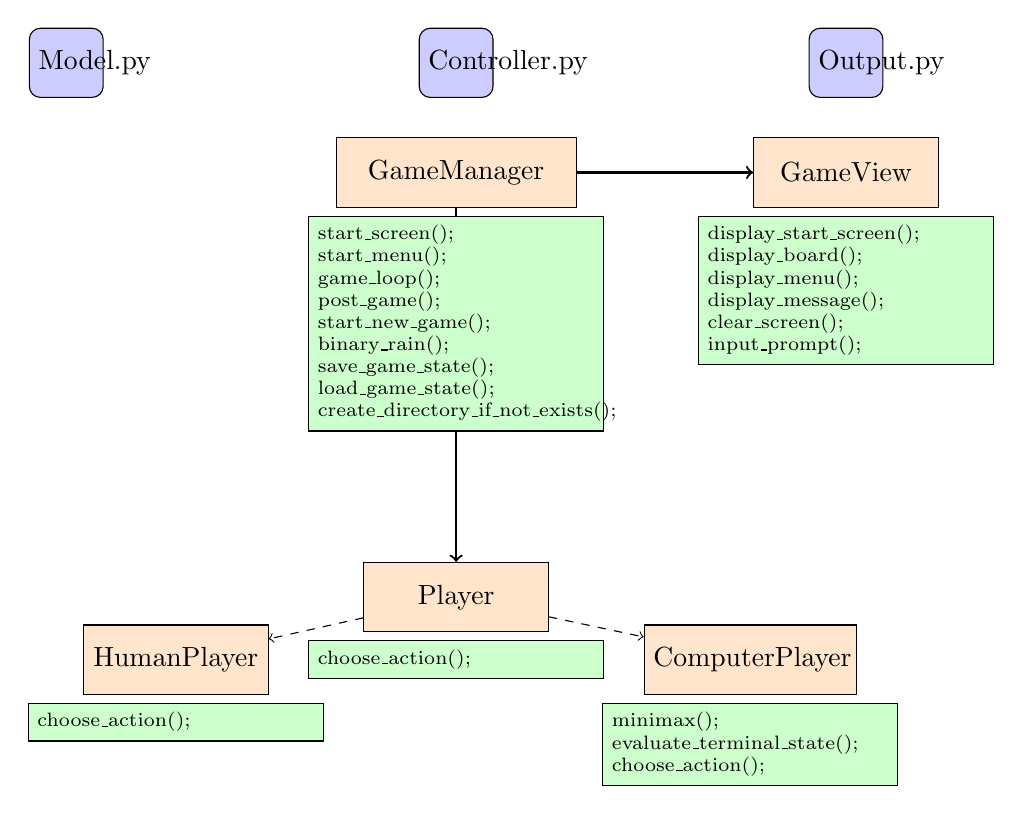
\begin{tikzpicture}[
  file/.style={draw, fill=blue!20, rectangle, rounded corners, text width=2em, align=center, minimum height=2.5em},
  class/.style={draw, fill=orange!20, rectangle, text width=6em, align=center, minimum height=2.5em},
  method/.style={draw, fill=green!20, rectangle, text width=10em, align=left, font=\scriptsize, anchor=north},
  inherit/.style={->, dashed},
  assoc/.style={->, thick}
]

% Files
\node[file] (Controller) {Controller.py};
\node[file, right=4cm of Controller] (Output) {Output.py};
\node[file, left=4cm of Controller] (Model) {Model.py};

% Classes under Controller.py
\node[class, below=0.5cm of Controller, text width=8em] (GameManager) {GameManager};
\node[method, below=0.1cm of GameManager] (GameManagerMethods) {
start\_screen();\\
start\_menu();\\
game\_loop();\\
post\_game();\\
start\_new\_game();\\
binary\_rain();\\
save\_game\_state();\\
load\_game\_state();\\
create\_directory\_if\_not\_exists();
};

% Classes under Output.py
\node[class, below=0.5cm of Output] (GameView) {GameView};
\node[method, below=0.1cm of GameView] (GameViewMethods) {
display\_start\_screen();\\
display\_board();\\
display\_menu();\\
display\_message();\\
clear\_screen();\\
input\_prompt();
};

\node[class, below=4.5cm of GameManager] (Player) {Player};
\node[method, below=0.1cm of Player] (PlayerMethods) {choose\_action();};

\node[class, left=0.5cm of PlayerMethods] (HumanPlayer) {HumanPlayer};
\node[method, below=0.1cm of HumanPlayer] (HumanPlayerMethods) {choose\_action();};

\node[class, right=0.5cm of PlayerMethods, text width=7em] (ComputerPlayer) {ComputerPlayer};
\node[method, below=0.1cm of ComputerPlayer] (ComputerPlayerMethods) {
minimax();\\
evaluate\_terminal\_state();\\
choose\_action();
};

% Inheritance relationships
\draw[inherit] (Player) -- (HumanPlayer);
\draw[inherit] (Player) -- (ComputerPlayer);

% Associations
\begin{pgfonlayer}{background}
%\draw[assoc] (GameManager) -- (GameBoard);
\draw[assoc] (GameManager) -- (GameView);
\draw[assoc] (GameManager) -- (Player);
\end{pgfonlayer}

\end{tikzpicture}

\newpage

\section{Serialization and Deserialization}
Serialization and deserialization mechanisms are crucial for saving and loading game states. This functionality is implemented through Python's JSON module, allowing game states to be saved to disk and retrieved later.

\subsection{Implementation Details}
Here we would provide code snippets showing how the game state is serialized into JSON format and deserialized back into game objects.

% Example code snippet
\begin{lstlisting}[language=Python, caption=Serialization Example]
import json

def save_game_state(self):
    game_state = {
        'board': self.board.board,
        'num_players': self.num_players,
        'current_turn': self.board.current_player()
    }
    with open(filename, 'w') as file:
        json.dump(game_state, file)
\end{lstlisting}

\section{Game AI}
The game AI uses the Minimax algorithm to determine the optimal move for the computer player. It evaluates the game board at each step to make the most advantageous move.

\subsection{Minimax Algorithm}
The Minimax algorithm is a recursive algorithm used for minimizing the possible loss for a worst-case scenario. When dealing with gains, it is maximizing the minimum gain.

\section{Tests}
Our testing strategy focused on achieving high code coverage and ensuring the reliability of the game's core functionalities. We utilized a combination of unit tests and integration tests.

\subsection{Achieving 90\% Line Coverage}
To ensure that at least 90\% of our business logic was covered by tests, we employed the following strategies:
\begin{itemize}
    \item Writing unit tests for all models and utility functions.
    \item Implementing integration tests to cover scenarios involving user interactions.
\end{itemize}

\section{Contributions}
This section details the contributions of each team member to the project. For example, John Doe was responsible for implementing the game AI, while Jane Doe focused on the serialization/des


\end{document} % This line is crucial